\subsection{Code generator}
As soon as a language is defined, for example by writing it down in \ac{EBNF}, the development of a code generator can be started. Generators can be implemented using a template-based approach \parencite[see][]{cleaveland_program_2001}, the template metaprogramming capabilities of a language (e.g., in C++), or extendable programming systems (e.g., OpenC++) \parencite[cf.][p. 16]{czarnecki_generative_2000}.\\
A code generator generally consists of several different phases or components, as shown in the following figure.
\begin{figure}[H]
    \caption{Code Generation Processing Phases}
    \label{fig:generator-process}
    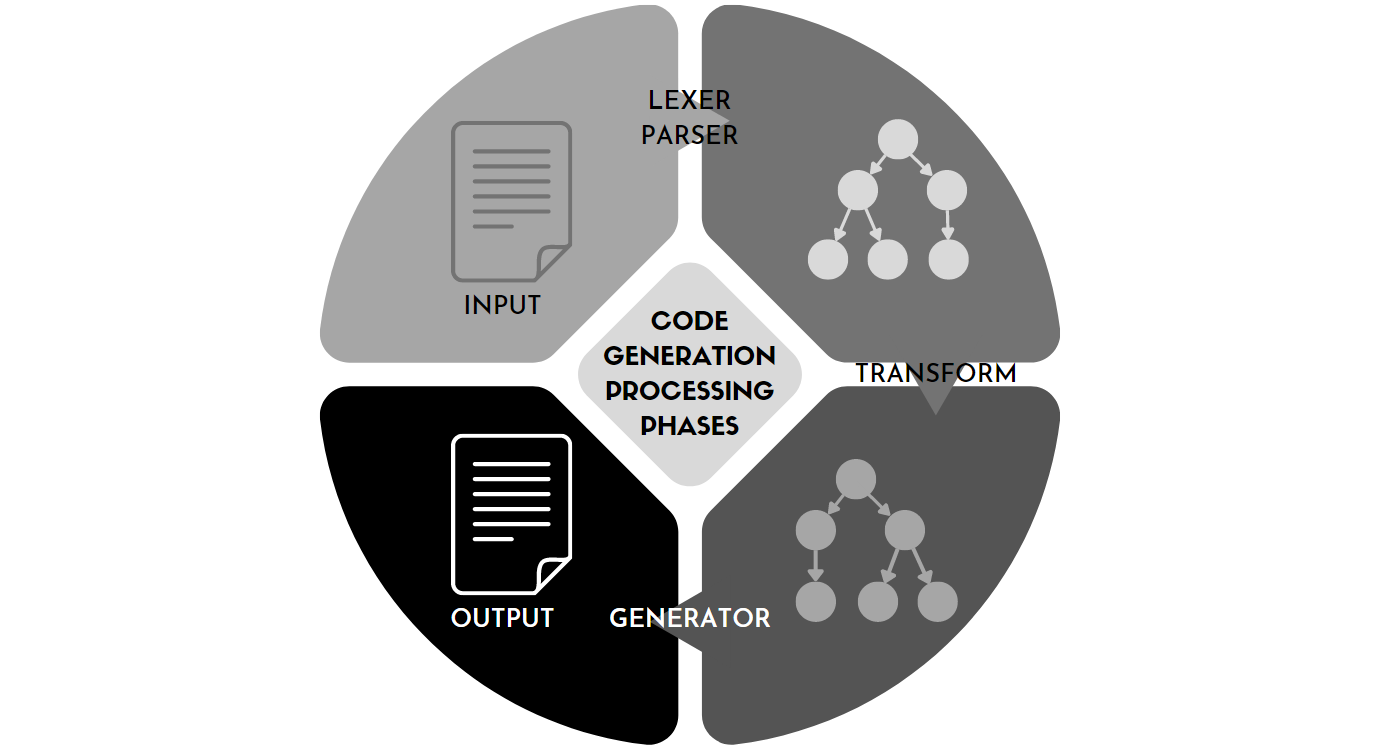
\includegraphics[width=0.9\textwidth]{generator-process.png}
    \\
    \cite[Source: Based on][p. 5]{sarkar_code_2001}
\end{figure}
A program written by a developer in either a predefined \ac{DSL} or an executable model is stored in a file for development. The code generator is given the grammar of the source language, which it uses to split it into tokens and then relate them to each other by parsing them. Such dependencies can also exist between multiple input files, by importing or referencing each other. The parser then arranges them in an \ac{AST}, which can be optimized and transformed for the target language. The generator or writer then generates a file in the target language from this \ac{AST}.\\
The code generator built in this thesis makes use of a lexer that takes care of the first initial step of scanning. Scanning is a good starting point and the first step in any compiler or interpreter. It takes the input file and groups a series of characters into so-called tokens. These words or punctuation make up the grammar of the query language \parencite[cf.][p. 39]{nystrom_crafting_2021}.\\
Keywords and many other special kinds of tokens are almost always part of a grammar of a language and have to be handled separately from other tokens, to achieve that tokens must be assigned a kind to differentiate them. Each keyword, operator, punctuation, and literal type are some kind of token \parencite[cf.][p. 43]{nystrom_crafting_2021}. Tokens can be recognized either by simply matching them to a character like '(' which would be then recognized as a left parenthesis token or if a token is more complex logic like if statements or regex can be used to further distinguish tokens \parencite[see][pp. 47-54]{nystrom_crafting_2021}.\\
The next goal is a transformation of the series of tokens into a more complex in-memory representation that can be used by an interpreter or, in the case of the thesis, a generator. This representation should be simple to generate for the parser and easy to understand for the next component \parencite[cf.][p. 59]{nystrom_crafting_2021}.\\
There exist two different types of parsers, namely, the event-driven parser and the tree-constructing parser \parencite[cf.][p. 5]{sarkar_code_2001}. Event-driven parsers search the input file for predefined syntax structures and notify the user when one is found. The user can then decide which events to ignore and which to include in their data structure. Tree constructors document related tokens as an \ac{AST}. Thus, this \ac{AST} contains an in-memory representation of the input files on which all further processing algorithms are based. If several languages and grammars are parsed several \ac{AST}s can develop \parencite[cf.][pp. 5-6]{sarkar_code_2001}.\\
In the context of the thesis, a tree-constructing parser is implemented which will be based on a previously defined grammar. The use of a notation such as \ac{EBNF}, described in chapter \ref{sec:EBNF}, helps silhouetting the informal syntax design and can serve as a guide when implementing the parser \parencite[cf.][p. 64]{nystrom_crafting_2021}.\\
In the implementation of the parser, many types of so-called expressions are needed to define parts of the language. For example, there are literal expressions, which represent elementary values, such as numbers, booleans, or strings, and binary expressions, which logically connect two other expressions with an operator. These different types of expressions are to be recognized by the parser and sorted accordingly into the tree structure \parencite[see][pp. 64-68]{nystrom_crafting_2021}.\\
With expressions alone, it is possible to correctly process the syntax for inputs like $1 * (2 - 3) == true$ according to their respective priority \parencite[cf.][p. 64]{nystrom_crafting_2021}.\\
Statements \parencite[see][pp. 111-116]{nystrom_crafting_2021}